% 图 81.6 —— 由 `checks/emit_hand.py` 自动拼出（probe 精测 + prims2 图元分解）
%%
% ⚠ 这是**稿子不是成品**：跑 `checks/checkhand.py 81.6` 看指标 + 看叠合图。
%%
%% ⚠ 待核：
%   · 本图 probe 报出阴影族 1 个 —— **本脚本不生成阴影**（要照原书手写）；prims2 的 strokes 里可能含阴影线，核对时留意别画重
%   · 可疑字形 1 项（空心圈 ⊙ 常被认成字母 o）—— 见文件末
%%
\documentclass[12pt]{standalone}
\usepackage{fontspec}
\setsansfont{Arial}
\newfontfamily\mfallback{DejaVu Sans}
\usepackage{tikz}
\begin{document}
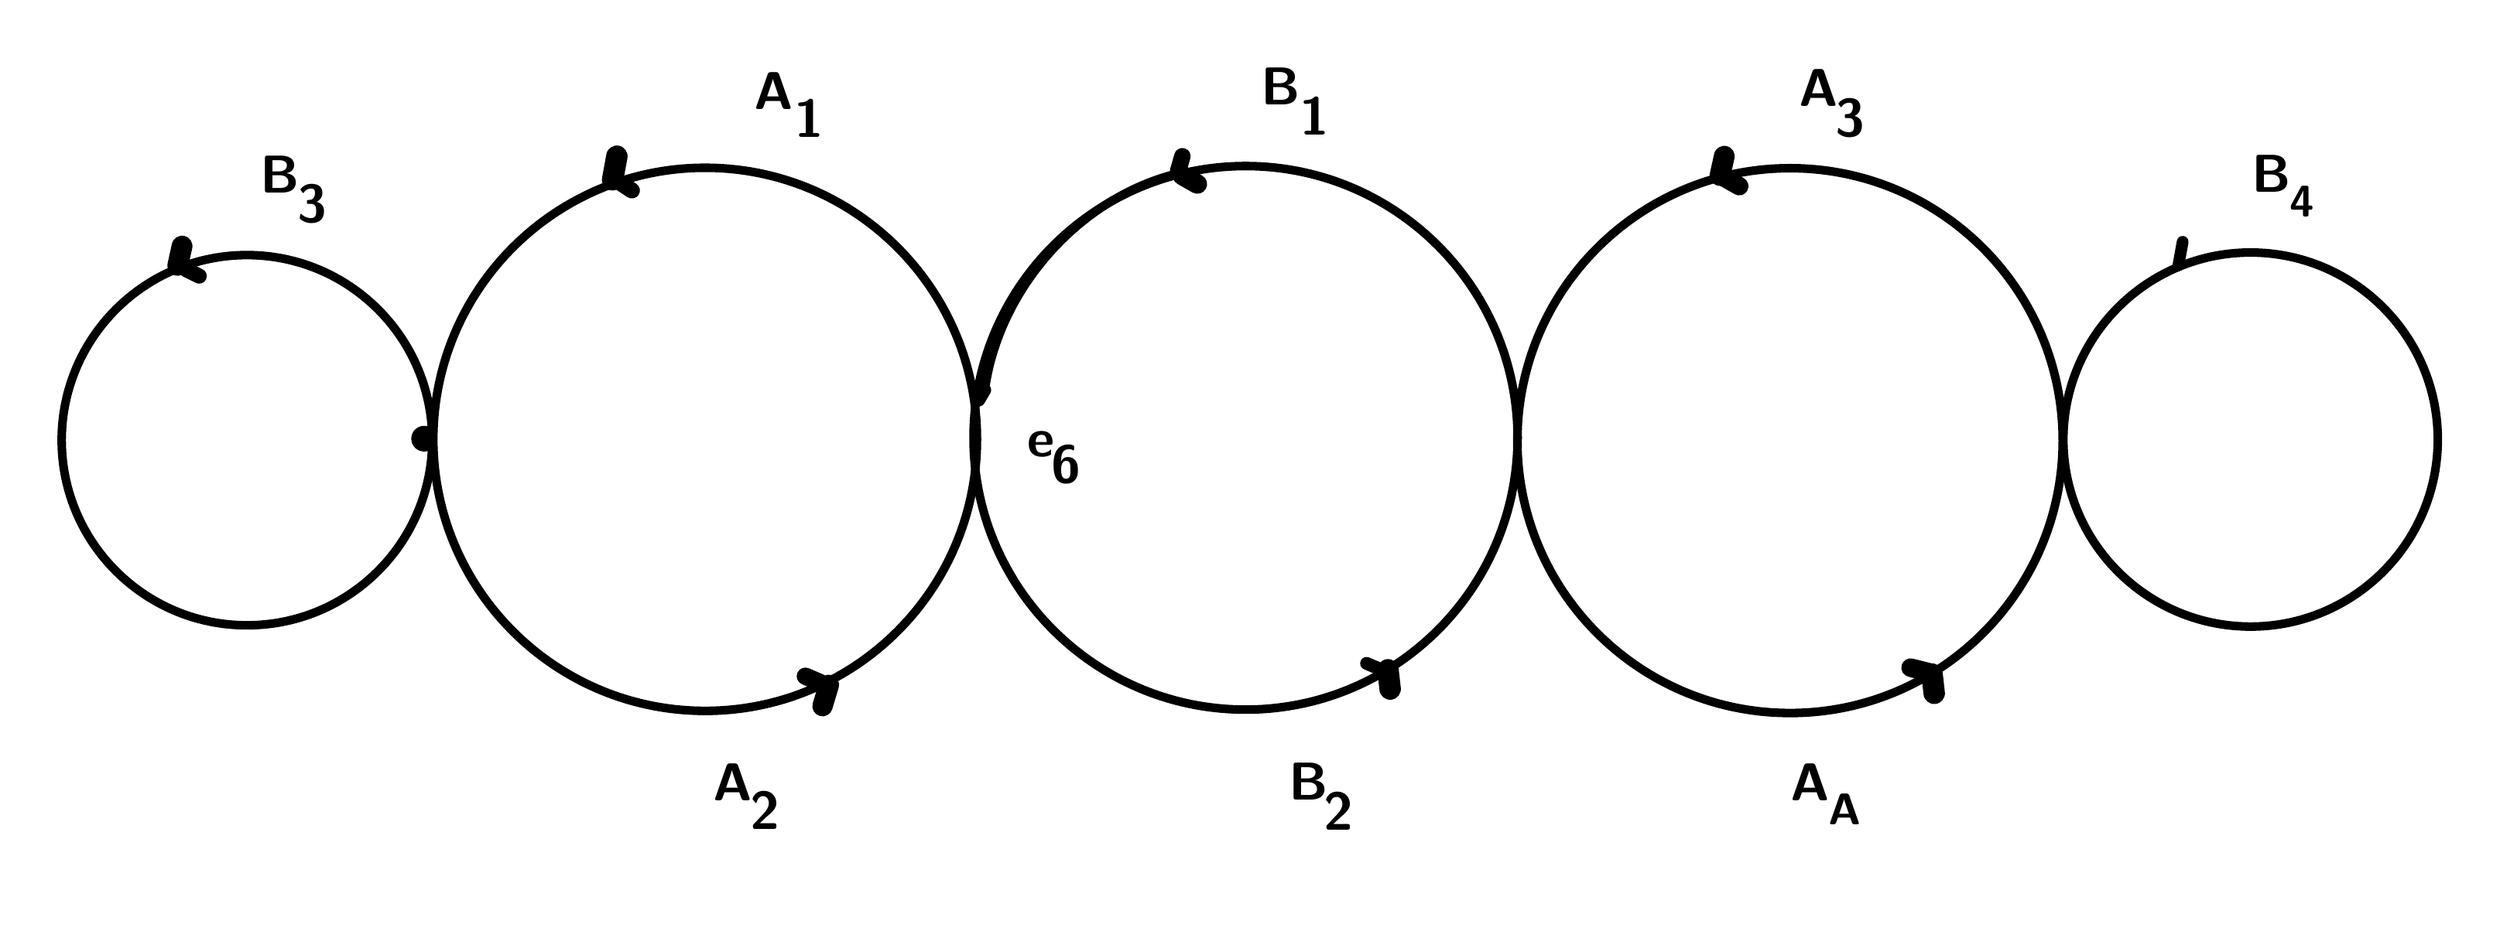
\begin{tikzpicture}[x=1pt, y=-1pt, line width=4.0pt, line cap=round, line join=round]

  %% ════ 填充区（prims2 的 fills）════

  %% ════ 直线段（prims2 的 strokes）════
  \draw[line width=8.6pt] (795.0,73.0) -- (802.0,77.0);
  \draw[line width=9.7pt] (793.0,72.0) -- (795.0,63.0);
  \draw[line width=7.7pt] (540.0,70.0) -- (542.0,63.0);
  \draw[line width=8.1pt] (373.0,309.0) -- (366.0,306.0);
  \draw[line width=10.0pt] (278.0,63.0) -- (276.0,74.0);
  \draw[line width=5.5pt] (1009.0,103.0) -- (1007.0,114.0);
  \draw[line width=9.1pt] (549.0,76.0) -- (542.0,72.0);
  \draw[line width=8.7pt] (882.0,302.0) -- (890.0,304.0);
  \draw[line width=9.5pt] (377.0,310.0) -- (374.0,320.0);
  \draw[line width=7.5pt] (279.0,75.0) -- (285.0,79.0);
  \draw[line width=10.0pt] (893.0,314.0) -- (892.0,305.0);
  \draw[line width=7.1pt] (83.0,119.0) -- (77.0,116.0);
  \draw[line width=10.0pt] (638.0,303.0) -- (639.0,312.0);
  \draw[line width=9.7pt] (75.0,105.0) -- (73.0,114.0);
  \draw[line width=5.9pt] (449.8,172.2) -- (447.0,177.0);
  \draw[line width=6.0pt] (628.0,300.0) -- (635.0,303.0);

  %% ════ 曲线（prims2 的 curves —— 三段式，坐标同为 (y,x)）════
  \draw[line width=4.0pt] (540.0,71.0) .. controls (493.9,82.3) and (456.2,125.0) .. (449.8,172.2);

  %% ════ 圆 / 椭圆（probe 精测）════
  \draw (825.7,195.9) circle (127.3);
  \draw (571.5,194.6) circle (127.0);
  \draw (319.2,195.3) circle (126.9);
  \draw (105.3,195.7) circle (86.5);
  \draw (1040.7,195.4) circle (87.4);

  %% ════ 实心点 ════
  \fill (188.0,195.0) circle (6.0);

  %% ════ 标签（probe 直接给的 \node 行）════
  %% ⚠ 全部补了 fill=white：文字在最上层，否则与曲线交叉干扰
     \node[anchor=center,inner sep=0pt,fill=white,font=\fontsize{30.3}{37.9}\selectfont] at (587.8,30.5) {\textsf{\textbf{\textit{B}}}};   % box(576,19,20,22)
     \node[anchor=center,inner sep=0pt,fill=white,font=\fontsize{28.9}{36.1}\selectfont] at (839.1,31.0) {\textsf{\textbf{\textit{A}}}};   % box(827,20,19,21)
     \node[anchor=center,inner sep=0pt,fill=white,font=\fontsize{29.6}{37.0}\selectfont] at (351.2,32.5) {\textsf{\textbf{\textit{A}}}};   % box(339,21,19,22)
     \node[anchor=center,inner sep=0pt,fill=white,font=\fontsize{23.7}{29.7}\selectfont] at (603.8,44.4) {\textsf{\textbf{1}}};   % box(597,36,8,16)
     \node[anchor=center,inner sep=0pt,fill=white,font=\fontsize{23.0}{28.7}\selectfont] at (853.9,45.1) {\textsf{\textbf{3}}};   % box(848,36,11,17)
     \node[anchor=center,inner sep=0pt,fill=white,font=\fontsize{23.7}{29.7}\selectfont] at (367.8,45.4) {\textsf{\textbf{1}}};   % box(361,37,8,16)
     \node[anchor=center,inner sep=0pt,fill=white,font=\fontsize{30.2}{37.8}\selectfont] at (1050.3,71.0) {\textsf{\textbf{\textit{B}}}};   % box(1039,59,19,23)
     \node[anchor=center,inner sep=0pt,fill=white,font=\fontsize{30.3}{37.9}\selectfont] at (120.8,71.5) {\textsf{\textbf{\textit{B}}}};   % box(109,60,20,22)
     \node[anchor=center,inner sep=0pt,fill=white,font=\fontsize{23.0}{28.7}\selectfont] at (135.9,85.1) {\textsf{\textbf{3}}};   % box(130,76,11,17)
     \node[anchor=center,inner sep=0pt,fill=white,font=\fontsize{20.8}{26.0}\selectfont] at (1064.7,84.3) {\textsf{\textbf{4}}};   % box(1059,76,10,16)
     \node[anchor=center,inner sep=0pt,fill=white,font=\fontsize{32.4}{40.5}\selectfont] at (475.9,197.6) {\textsf{\textbf{\textit{e}}}};   % box(466,187,16,18)
     \node[anchor=center,inner sep=0pt,fill=white,font=\fontsize{24.4}{30.5}\selectfont] at (487.6,207.1) {\textsf{\textbf{6}}};   % box(481,198,12,17)
     \node[anchor=center,inner sep=0pt,fill=white,font=\fontsize{31.0}{38.8}\selectfont] at (600.8,355.0) {\textsf{\textbf{\textit{B}}}};   % box(589,343,20,23)
     \node[anchor=center,inner sep=0pt,fill=white,font=\fontsize{29.6}{37.0}\selectfont] at (332.2,355.5) {\textsf{\textbf{\textit{A}}}};   % box(320,344,19,22)
     \node[anchor=center,inner sep=0pt,fill=white,font=\fontsize{29.6}{37.0}\selectfont] at (835.2,355.5) {\textsf{\textbf{\textit{A}}}};   % box(823,344,19,22)
     \node[anchor=center,inner sep=0pt,fill=white,font=\fontsize{23.6}{29.6}\selectfont] at (347.1,368.9) {\textsf{\textbf{2}}};   % box(341,360,11,17)
     \node[anchor=center,inner sep=0pt,fill=white,font=\fontsize{19.2}{24.0}\selectfont] at (851.3,368.3) {\textsf{\textbf{\textit{A}}}};   % box(844,360,11,16)
     \node[anchor=center,inner sep=0pt,fill=white,font=\fontsize{22.9}{28.7}\selectfont] at (615.1,369.4) {\textsf{\textbf{2}}};   % box(609,361,11,16)

  % 钉死画布：否则超出的图元/控制点会把页面撑大，1:1 回比就失准
  \pgfresetboundingbox
  \path[use as bounding box] (0,0) rectangle (1147,415);
\end{tikzpicture}
\end{document}

% ⚠ 待核清单（probe 拿不准，人眼过一遍）：
%   · 未识别/跳过：⑤ 跳过/未识别的字形
